% UQ Gemini theme
% See: https://github.com/alfurka/gemini-uq
% Forked from
% https://rev.cs.uchicago.edu/k4rtik/gemini-uccs
% which is forked from
% https://github.com/anishathalye/gemini


\documentclass[final,xcolor=table]{beamer}

% ====================
% Packages
% ====================

\usepackage[T1]{fontenc}
\usepackage{lmodern}
\usepackage[size=custom,width=100,height=75,scale=1.0]{beamerposter}
\usetheme{gemini}
\usecolortheme{uchicago}
\usepackage{graphicx}
\usepackage{booktabs}
\usepackage{tikz}
\usepackage{pgfplots}
\pgfplotsset{compat=1.17}
\usepackage{tabularx}
\usepackage{adjustbox}
\usepackage{hyperref}

\definecolor{mycolor}{HTML}{000AFC}
\hypersetup{
    colorlinks=true,
    urlcolor=mycolor
    }

% ====================
% Lengths
% ====================

% If you have N columns, choose \sepwidth and \colwidth such that
% (N+1)*\sepwidth + N*\colwidth = \paperwidth
\newlength{\sepwidth}
\newlength{\colwidth}
\setlength{\sepwidth}{0.03\paperwidth}
\setlength{\colwidth}{0.45\paperwidth}

\newcommand{\separatorcolumn}{\begin{column}{\sepwidth}\end{column}}

% ====================
% Title
% ====================

\title{Air Quality Forecast and Dispersion Outlook of \\Allegheny County, Pennsylvania}

\author{03/30/2022}
\institute[shortinst]{\inst{1} Some Institute \samelineand \inst{2} Another Institute}
% ====================
% Footer (optional)
% ====================

\footercontent{
  \href{https://www.example.com}{https://www.alleghenycounty.us/Health-Department/Programs/Air-Quality/Air-Quality.aspx} \hfill
  Allegheny County \hfill
  \href{mailto:a.kalay@example.com}{412-687-2243}}
% (can be left out to remove footer)

% ====================
% Logo (optional)
% ====================

% use this to include logos on the left and/or right side of the header:
% \logoright{\includegraphics[height=7cm]{logo1.pdf}}
% \logoleft{\includegraphics[height=7cm]{logo2.pdf}}

% ====================
% Body
% ====================

\begin{document}
\addtobeamertemplate{headline}{}
{
    \begin{tikzpicture}[remember picture,overlay]
      \node [anchor=north west, inner sep=3.5cm] at ([xshift=-2cm,yshift=2.5cm]current page.north west)
      {
\includegraphics[height=2.5cm]{logos/allegheny.png}}; % also try shield-white.eps
      \node [anchor=north east, inner sep=3cm] at ([xshift=0.0cm,yshift=2.5cm]current page.north east)
      {
\includegraphics[height=8.0cm]{logos/achd.png}};
    \end{tikzpicture}
}

\begin{frame}[t]
\begin{columns}[t]
\separatorcolumn

\begin{column}{\colwidth}

  \begin{block}{Air Quality Forecast}

    This is the daily forecasted Air Quality Index (AQI) for each area provided by the PA Department of Environmental Protection. The AQI is based on PM2.5 or Ozone, whichever is forecasted to be higher.

    \begin{table}
      \renewcommand{\arraystretch}{1.5}
      \centering
      \begin{tabular}{|c| c| c|}
        \hline
        \rowcolor{lightgray}\textbf{Forecast Period} & \textbf{Pittsburgh Area} & \textbf{Liberty-Clairton Area} \\
        \hline
        \rowcolor[HTML]{F2FDFE}{Today} & {\textbf{Moderate} 51 AQI} & {\textbf{Moderate} 53 AQI} \\
        \hline
        \rowcolor[HTML]{F2FDFE}Tomorrow & {\textbf{Good} 38 AQI} & {\textbf{Good} 36 AQI} \\
        \hline
      \end{tabular}
      \caption{Please refer the Air Quality Index guide}
    \end{table}

    \heading{Today’s Forecast:}
    Much warmer air will stream into the area Wednesday with sunshine returning by the afternoon as winds turn into the south-southeast. PM2.5 will rise some Wednesday, perhaps into the moderate range as a moderate to strong inversion is likely during the morning, with better air quality occurring during the afternoon.
    

    \begin{table}
      \begin{adjustbox}{width=1\textwidth}
      \renewcommand{\arraystretch}{1.5}
      \centering
      \begin{tabular}{|c |c |c |c|}
      \hline
      \rowcolor{lightgray}\multicolumn{4}{|c|}{\textbf{Guide to the Air Quality Index (AQI)}} \\
      \hline
      \rowcolor{lightgray}\textbf{Color} & \textbf{Description} & \textbf{Meaning} & \textbf{AQI} \\
      \hline
      \rowcolor[HTML]{F2FDFE}{\cellcolor[HTML]{FF2121}\textbf{Red}} & Unhealthy & Everyone should limit exertion outdoors. & 151 - 200 \\
      \rowcolor[HTML]{F2FDFE}{\cellcolor[HTML]{FF6A20}\textbf{Orange}} & Unhealthy for Sensitive Groups & Sensitive people should limit exertion outdoors. & 101 - 150 \\
      \rowcolor[HTML]{F2FDFE}{\cellcolor[HTML]{FFF421}\textbf{Yellow}} & Moderate & Extremely sensitive people may wish to limit outdoor exertion. & 51 - 100 \\
      \rowcolor[HTML]{F2FDFE}{\cellcolor[HTML]{6AFE19}\textbf{Green}} & Good & No health impacts are expected in this range. & 0 - 50 \\
      \hline
      \end{tabular}
      \end{adjustbox}
    \end{table}

    \href{https://www.ahs.dep.pa.gov/AQPartnersWeb/forecast_home.aspx}{\underline{Data provided by the PA Department of Environmental Protection}}

  \end{block}

  \begin{block}{ACHD Air Dispersion 36-Hour Forecast}

    This is the dispersion forecast for Allegheny County starting from this morning through tomorrow afternoon. The atmospheric dispersion index is a rating of the atmosphere’s ability to transport pollution away from its source and is based on emissions and weather. Better atmospheric dispersion can improve air quality.

    \begin{table}
      \renewcommand{\arraystretch}{1.5}
      \centering
      \begin{adjustbox}{width=1\textwidth}
      \begin{tabular}{ |c|c|c|c|c|}
          \hline
          \rowcolor{lightgray}\multicolumn{2}{|c|}{\textbf{Forecast Period}} & \textbf{Atmospheric Dispersion Index} & \textbf{Surface Inversion Strength} & \textbf{Wind (dir, mph)}\\
          \hline
          \rowcolor[HTML]{F2FDFE}{\textbf{Today}} & Morning & Poor–8 & Slight & ESE 7-8 to SE 8-9 \\ 
          \rowcolor[HTML]{F2FDFE} & Afternoon & Generally Good–46 & -- & SE 9-11 \\
          \hline
          \rowcolor[HTML]{F2FDFE}{\textbf{Tonight}} & Evening  & Poor–12 & -- & SE 9-10 to SSE 10-11 Gust 20-21\\
          \rowcolor[HTML]{F2FDFE} & Overnight & Generally Poor–18 & -- & S 11-14 Gust 21-28\\
          \hline
          \rowcolor[HTML]{F2FDFE}{\textbf{Tomorrow}} & Morning & Generally Good–44 & None & SSW 14-15 to SW 15-17 Gust 25-34\\
          \rowcolor[HTML]{F2FDFE} & Afternoon & Very Good-136 & -- & SW 17-18 to W 11 Gust 21-35\\
          \hline
      \end{tabular}
      \end{adjustbox}
      \caption{Please refer the Atmospheric Dispersion Index guide and the daily Surface Temperature Inversion Report.}
    \end{table}

    \heading{ACHD Remarks:}
    Chance of rain this morning and rain likely tomorrow. Also, the sounding data from the National Weather Service was unavailable, so I had to use an alternative source.
    
    Data provided by the National Weather Service (NWS)
    \href{https://forecast.weather.gov/product.php?site=NWS&product=FWF&issuedby=PBZ}{\underline{Fire Weather Planning Forecast}} and \href{http://weather.uwyo.edu/upperair/sounding.html}{\underline{PIT NWS Products}}

  \end{block}
  
\end{column}

\separatorcolumn

\begin{column}{\colwidth}

    \begin{table}
      \renewcommand{\arraystretch}{1.5}
      \centering
        \begin{tabular}{ |c |c |c |c|c |c |c|  }
        \hline
        \rowcolor{lightgray}\multicolumn{7}{|c|}{\textbf{Guide to the Atmospheric Dispersion Index}} \\
        \hline
        \rowcolor[HTML]{F2FDFE}\textbf{Very Poor} & \textbf{Poor} & \textbf{Generally Poor} & \textbf{Fair} & \textbf{Generally Good} & \textbf{Good} & \textbf{Very Good} \\
        \hline
        \rowcolor[HTML]{F2FDFE}1 - 6 & 7 - 12 & 13 - 20 & 21 - 40 & 41 - 60 & 61 - 100 & > 100 \\
        \hline
        \end{tabular}
    \end{table}


  \begin{block}{ACHD Surface Temperature Inversion Report}

    \textit{This is the 7 AM surface-based temperature inversion report for Allegheny County.}

    This morning’s surface inversion of \underline{\textbf{~0.59 °C}} with a depth of \underline{\textbf{~60}} m is estimated to break at \underline{\textbf{N/A}} . This surface inversion can be characterized as: None/ \underline{\textbf{Slight}} / Weak / Moderate / Strong. No upper inversion starting below ~1000 m is reported.

  \end{block}

  \begin{block}{What does the Surface Temperature Inversion Report mean}

    A surface temperature inversion is a weather pattern that stops mixing of the air near the ground, and pollution released into the air tends to remain at higher concentrations.
    
    \begin{columns}[T]
    \begin{column}{0.43\linewidth}
    ~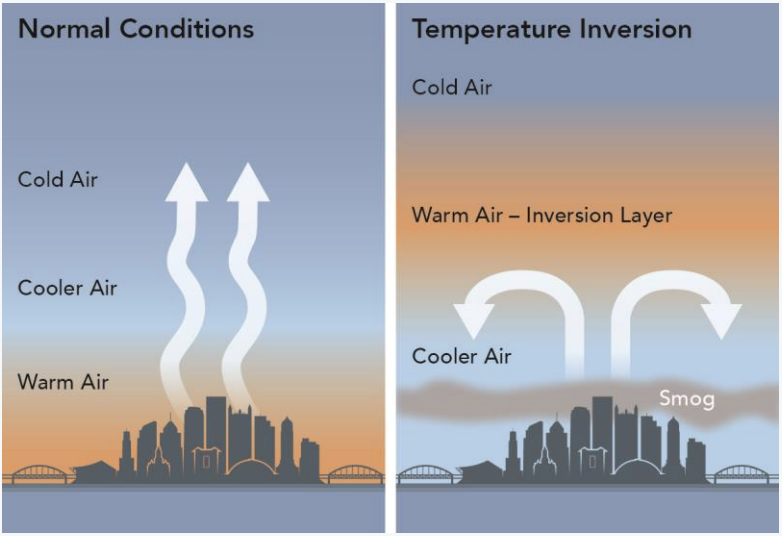
\includegraphics[width=1\textwidth]{citypic.png}
    \end{column}
    \begin{column}{0.5\linewidth}
    
        Surface temperature inversion conditions include how strong the surface inversion is (in °C), how high the inversion is above the surface (in meters), and when the inversion is expected to break (in Eastern Standard Time). Also included is whether an upperlevel inversion or inversions exist, starting at about 1,000 meters.
        
        \textbf{Surface Temperature Inversion Characterization}
            \begin{itemize}
              \item 0-0.9 C°: Slight
              \item 1-2.9 C°: Weak
              \item 3-4.9 C°: Moderate
              \item ≥5 C°: Strong
            \end{itemize}
    \end{column}
    \end{columns}    


  \end{block}



  \begin{block}{References}

    \nocite{*}
    \footnotesize{\bibliographystyle{plain}\bibliography{poster}}

  \end{block}

\end{column}

\separatorcolumn
\end{columns}
\end{frame}
\end{document}
